\chapter{Query Facet Extraction}
\label{ch:facet}
\section{Introduction}
In conventional faceted search, facets are generated in advance for an entire corpus~\cite{stoica2007automating,dakka2008automatic} either manually or semi-automatically, and then recommended for particular queries in most of the previous work~\cite{teevan2008challenges}. However, this approach is difficult to extend to faceted web search due to the large and heterogeneous nature of the web: because the web is very large, it is
difficult to assign quality facets to every document in the collection and to retrieve the full set of search results and their associated facets at query time; and because the web is heterogeneous, it is difficult to apply the same facets to every search result or every query.

To cope with this challenge, in this chapter, we propose an alternative solution, called \textbf{query facet extraction}~\cite{kong2013extracting}, which extracts facets for queries from their web search results. For example, when users search with the query \concept{baggage allowance}, the system might extract query facets like airlines, \{\concept{Delta}, \concept{JetBlue}, \concept{AA}, ...\}, travel classes, \{\concept{first}, \concept{business}, \concept{economy}\}, and flight types, \{\concept{international}, \concept{domestic}\}. Changing from a global approach that generates facets in advance for an entire corpus to a query-based approach that extract facets from the top-ranked search results, query facet extraction appears to be a promising direction for solving the open-domain faceted search problem -- it not only makes the facet generation problem easier, but also addresses the facet recommendation problem at the same time.


We define a \textbf{query facet} as a set of coordinate terms (\eg, \{\concept{AA}, \concept{Delta}, \concept{JetBlue},...\}) that explicitly represent one aspect (\eg, \concept{airlines}) of its query (\eg, \concept{baggage allowance}). The coordinate terms share a semantic relationship by being subsumed by a more general hypernym (\eg, \concept{AA}, \concept{Delta}, \concept{JetBlue} are subsumed by \concept{airlines}). 
% Terms in query facet are generally called \textbf{facet terms}. When it is clear from context, we will simply use ``facet'' for ``query facet'', and ``term'' for ``facet term'' for convenience. Based on these definitions, \textbf{query facet extraction} is to extract query facets for a given query from certain resources, and in our case the top search results for that query.
In Table~\ref{tab:facet-facetexample}, we show query facets for three example queries. We will using the first query \concept{mars landing} as an example for explanation. The first query facet, \{\textit{Curiosity}, \textit{Opportunity}, \textit{Spirit}\}, includes different Mars rovers. The second query facet, \{\textit{USA}, \textit{UK}, \textit{Soviet Union}\}, includes countries relevant to Mars landings. The last facet, \{\textit{video}, \textit{pictures}, \textit{news}\}, includes different types of media. We can see that the terms in each facet are instances of the same semantic class.
\begin{table}[H]
\centering
\caption{Query facet examples for three queries}
\label{tab:facet-facetexample}
\begin{tabular}{|l|} \hline
Query 1: Mars landing \\\hline
Query Facet 1: Curiosity, Opportunity, Spirit \\
Query Facet 2: USA, UK, Soviet Union \\
Query Facet 3: video, pictures, news \\\hhline{|=|}
Query 2: baggage allowance \\\hline
Query Facet 1: AA, Delta, Jetblue,  ... \\
Query Facet 2: international, domestic \\
Query Facet 3: first class, business class, economy class \\
Query Facet 4: weight, size, quantity \\\hhline{|=|}
Query 3: Mr Bean \\\hline
Query Facet 1: comics, movies, tv, books \\
Query Facet 2: The Curse of Mr Bean, Mr Bean Goes to Town, ...\\
Query Facet 3: Rowan Atkinson, Richard Wilson, Jean Rochefort,  ...\\ 
Query Facet 4: Mr Bean, Irma gobb, Rupert, Hubert, ...\\\hline
\end{tabular}
\end{table}


In this work, we use query facet extraction to address the problem of facet generation in Faceted Web Search. This approach first extracts candidate facets from the top search results based on textual and HTML patterns, and then refines the extracted candidates, which are often very noisy, using clustering methods. We develop a supervised method based on a graphical model for refining facet candidates. The graphical model learns how likely it is that a term should be selected from the candidates and how likely it is that two terms should be grouped together in a query facet. Further, the model captures the dependencies between the two factors. We propose two algorithms for approximate inference on the graphical model since  exact inference is intractable. This proposed method can easily incorporate a rich set of features and learn from available human labels.
%Also, we design an evaluation metric for query facet extraction, which combines recall and precision of the facet term, with the grouping quality.
%The evaluation metrics will be discussed in Chapter~\ref{ch:intrinsiceval}.

The rest of this chapter is organized as follows. We first define the task of query facet extraction and related concepts in Section~\ref{sec:facet-task}, and then describe a general framework to solve this problem in Section~\ref{sec:facet-framework}. We propose a supervised clustering method based on a graphical model for refining extracted candidates in Section~\ref{sec:facet-gm}. Last, we describe other methods that can be used for refining extracted candidates, including topic modeling (e.g., pLSA, LDA) and a variation of quality threshold clustering model~\cite{dou2011finding} in Section~\ref{sec:facet-other}. 
%The work in this chapter is completed and published~\cite{kong2013extracting}.

\section{Task Description}
\label{sec:facet-task}
\subsection{Query Facet}
To differentiate our work with facets in conventional faceted search, we call typically facets for a particular query ``query facets''. A query facet is a set of coordinate terms -- i.e., terms that share a semantic relationship by being subsumed by a more general hypernym, and they succinctly represent different options in the same category that a user can select to refine the issued query. 

We call these terms inside a query facet ``facet terms'', which can be single words (e.g. \concept{international}, \concept{domestic} in Table~\ref{tab:facet-facetexample}) or phrases (e.g. \concept{first class}, \concept{business class} in Table~\ref{tab:facet-facetexample}).

This definition of query facets corresponds to a one-level faceted taxonomy, in which only information objects that belong to a same parent node are shown as a query facet (Section~\ref{sec:bg-fws}). We leave generating query facets as two or more level taxonomies to future work.

When it is clear from context, we will simply use ``facet'' for ``query facet'', and ``term'' for ``facet term'' for convenience.

\subsection{Query Facet Extraction}
Based on the definitions above, query facet extraction is to extract query facets for a given query from certain resources. While a variety of different resources can be used for query facet extraction, such as a query log, anchor text, taxonomy and social folksonomy, in this work, we only focus on extracting query facets from the top ranked web search results, and and leave others as future work.

\section{Solution Framework}
\label{sec:facet-framework}
% intuition and assumptions
The idea for solving query facet extraction is to leverage coordinate terms found in the web search results to build high-quality query facets. These coordinate terms can be found by looking into the list structures in webpages (\eg, ordered lists, drop-down lists) or analyzing the linguistic list structures in the textual content (\eg, \concept{The airlines servicing this airport are \underline{AA}, \underline{Delta}, and \underline{JetBlue}}).
Previous work in semantic class extraction~\cite{hearst1992automatic,pasca2004acquisition,kozareva2008semantic,shi2010corpus} has studied patterns for extracting these structures. 

This idea is based on the following two assumptions:
\begin{enumerate}[label={(\arabic*)}]
 \item The list structures consist of coordinate terms, or terms that share peer relationships. According to webpage design conversions, webpage editors often list peering information objects in the HTML list structures. Similarly, the linguistic list structures are often used to list peer information objects in writing.
 \item The list structures present relevant and important aspects of the query. Assuming the search results are relevant to the query, those list structures extracted from the search result should also be related to the query.  And, if they occur frequently, they may also be important to that query.
\end{enumerate}

Based on the idea, we develop the following general solution framework for query facet extraction, as also illustrated in Figure~\ref{fig:facet-framework}:
\vspace{+5mm}
\begin{figure}[ht!]
\centering
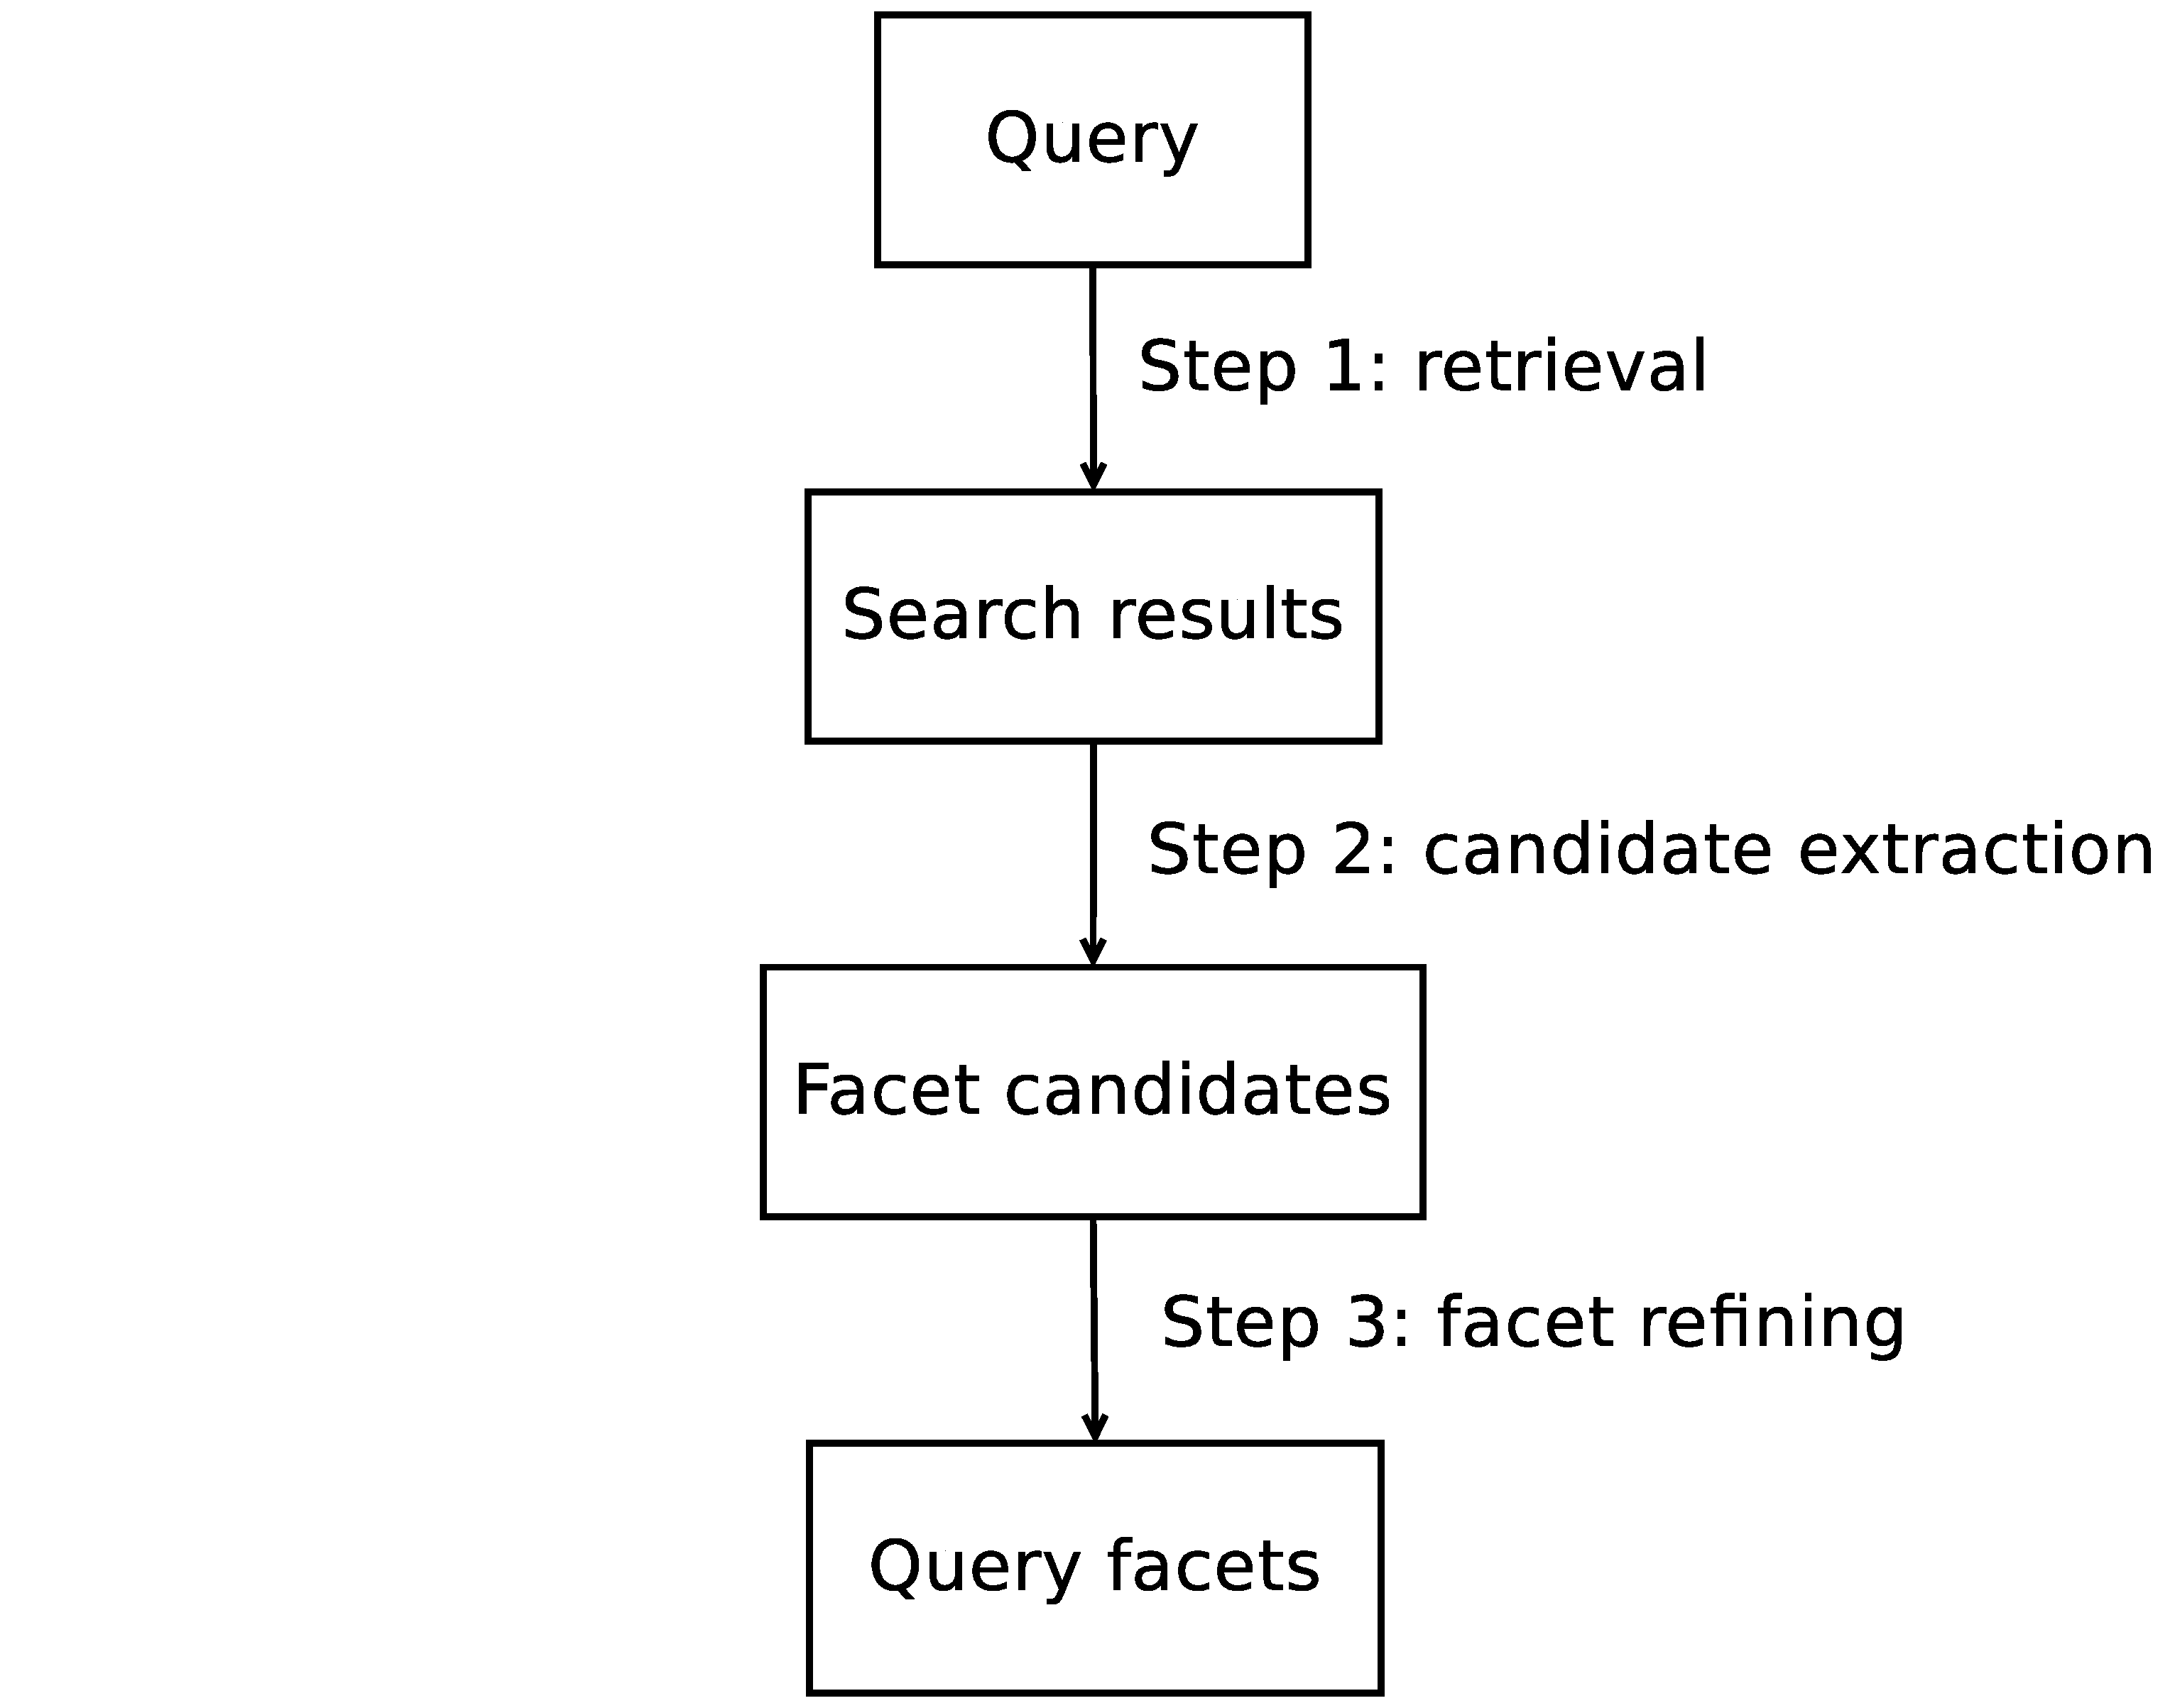
\includegraphics[width=0.75\columnwidth]{drawing/facet-solution.eps}
\caption{Query facet extraction framework}
\label{fig:facet-framework}
\end{figure}
\begin{enumerate}[label={(\arabic*)}]
 \item \textbf{Retrieval}: in the first step, given a query, we retrieve the top search results.
 \item \textbf{Candidate extraction}: in the second step, we extract list structures as facet candidates from the search results based on pre-defined extraction patterns.
 \item \textbf{Facet Refining}: the facet candidates extracted are often very noisy, and cannot be directly used as query facets. In the last step, we refine the candidates to final query facets by re-clustering facets or terms in the candidate set.
\end{enumerate}

We will describe candidate extraction and facet refining in more detail in the next two sections. 

\section{Candidate Extraction}
\label{sec:facet-candidate}
Following \citet{dou2011finding}, we use a pattern-based semantic class extraction approach~\cite{shi2010corpus} to extract lists of coordinate terms from search results as facet candidates. In pattern-based semantic class extraction, instances of a semantic class (\eg, instance \concept{AA}, \concept{Delta}, \concept{JetBlue} for class \concept{airlines}) are extracted from textual or webpage corpus based on lexical patterns~\cite{hearst1992automatic,pasca2004acquisition}, HTML patterns~\cite{shinzato2005simple}, or both~\cite{shi2008pattern,zhang2009employing}. For example, the pattern ``\textit{NP}, \textit{NP}, ..., and \textit{NP}'', where \concept{NP} stands for a noun phrase, can be used to extract coordinate terms (as instances) from text. Besides lexical patterns, HTML patterns are often used on HTML documents to extract coordinate terms from some HTML structures, like unordered lists (\ie, <UL>), drop-down lists (\ie, <SELECT>) and 
tables (\ie, <TABLE>). The coordinate terms extracted from each patterns form candidates for query facets, which we call \textbf{candidate list}.

We apply both of the two types of patterns on the search results to extract candidate lists. These extraction patterns are summarized in Table~\ref{tab:facet-patterns}. We describe them in detail in the following two sections.

\begin{table}[H]
\centering
\caption{Candidate list extraction patterns. All matched \textit{items} in each pattern are extracted as a candidate list.}
\label{tab:facet-patterns}
\begin{tabular}{|c|l|} \hline
Type& Pattern\\ \hline
Lexical & \textit{item}, \{,\textit{item}$\}^*$, (and|or) \{other\} \textit{item} \\  \hline
\multirow{4}{*}{HTML}
& <select><option>\textit{item}</option>...</select>\\\cline{2-2}
& <ul><li>\textit{item}</li>...</ul>\\\cline{2-2}
& <ol><li>\textit{item}</li>...</ol>\\\cline{2-2}
& <table><tr><td>\textit{item}<td>...</table>\\ \hline
\end{tabular}
\end{table}

\subsection{Lexical Patterns}
We use the following lexical pattern:
\begin{center}
\textit{item} \{,\textit{item}$\}^*$ \{,\} (and|or) \{other\} \textit{item} 
\end{center}
\todo{James' comments}We apply the pattern on the textual content (ignoring HTML tags and formatting in the webpage) of the search results, and extract matched \textit{items} as a candidate list. To give an example, for the sentence, \concept{The airlines servicing this airport are AA, Delta, and JetBlue
}, we can extract the candidate list \{\concept{AA}, \concept{Delta}, \concept{JetBlue}\} using the lexical pattern. For this lexical pattern, we also restrict those \textit{items} to be siblings in the parse tree of that sentence in order to improve extraction quality. We use the PCFG parser~\cite{klein2003accurate} implemented in Stanford CoreNLP~\cite{manning2014stanford} for parsing documents.

\subsection{HTML Patterns}
We also extract candidate lists based on several HTML patterns that target list structures in HTML webpages, including drop-down lists, ordered lists, unordered lists and tables. Table~\ref{tab:facet-html} shows some HTML code examples for these list structures.
\begin{table}[ht!]
\centering
\caption{HTML code examples for drop-down lists (SELECT), ordered lists (OL), unordered lists (UL) and tables (TABLE).} 
\label{tab:facet-html}
\begin{tabular}{|l|} \hline
SELECT \\\hline
<select>\\
<option value=``1''>first class</option>\\
<option value=``2''>business class</option>\\
<option value=``3''>economy class</option>\\
</select>\\\hline
OL \\\hline
<ol>\\
<li>checked baggage allowance</li>\\
<li>carry on baggage allowance</li>\\
<li>excess baggage allowance</li>\\
</ol>\\\hline
UL \\\hline
<ul> \\
<li><a href=``courtesy\_bags.aspx''>Courtesy bags</a></li>\\
<li><a href=``dangerous.aspx''>Dangerous goods</a></li>\\
<li><a href=``devices.aspx''>Electronic devices</a></li>\\
<li><a href=``sports.aspx''>Sports equipment</a></li>\\
</ul>\\\hline
TABLE \\\hline
<table>\\
\small{<tr><td></td><td>economy</td><td>business</td>first</tr>}\\
\small{<tr><td>domestic</td>2 bags</td><td>3 bags</td><td>4 bags</td></tr>}\\
\small{<tr><td>international</td>1 bag</td><td>2 bags</td><td>3 bags</td></t>}\\
</table>\\\hline
\end{tabular}
\end{table}

We extract those HTML list structures based on the HTML patterns listed in Table~\ref{tab:facet-patterns}. Note that we do not match the HTML patterns with the HTML code exactly. Instead, we parse the HTML page into objects and extract textual content in the tags that we are interested in. We describe the extraction in details below:
\begin{itemize}
 \item \textbf{SELECT}: For the SELECT tag, we extract textual content in the OPTION tags as a candidate lists. For the example in Table~\ref{tab:facet-html}, we will extract candidate list \{\concept{first class}, \concept{business class}, \concept{economy class}\}.
\item \textbf{OL}: For the OL tag, we extract textual content in the LI tags as a candidate lists. For the example in Table~\ref{tab:facet-html}, we will extract candidate list \{\concept{checked baggage allowance}, \concept{carry on baggage allowance}, \concept{excess baggage allowance}\}.
\item \textbf{UL}: Similarly, for the UL tag, we also extract textual content in the LI tags as a candidate lists. For the example in Table~\ref{tab:facet-html}, we will extract candidate list \{\concept{Courtesy bags}, \concept{Dangerous goods}, \concept{Electronic devices}, \concept{Sports equipment}\}. Note that in this case, when extracting textual content in the LI tags, we ignore other HTML tags/formatting (\ie, \concept{<a>}).
\item \textbf{TABLE}: for HTML tables, following \citet{dou2011finding}, we extract candidate lists from each columns and each rows. For the example in Table~\ref{tab:facet-html}, we will extract 7 candidate lists.
To list a few, \{\concept{economy}, \concept{business}, \concept{first}\} and \{\concept{domestic}, \concept{2 bag}, \concept{3 bags}, \concept{4 bags}\} are extracted from the first two rows. \{concept{domestic}, \concept{international}\} and \{\concept{economy}, \concept{2 bags}, \concept{1 bag}\} are extracted from the first two columns.
\end{itemize}


Ordered lists (OL) and unordered lists (UL) can be nested, as shown in Figure~\ref{fig:nestedlist}. For nested HTML lists, we extract all sibling items from each level. For the example in Figure~\ref{fig:nestedlist}, we will extract two lists,
\{\concept{Coffee}, \concept{Tea}, \concept{Milk}\} and \{\concept{Black tea}, \concept{Green tea}\}.
\begin{figure}[ht!]
\centering
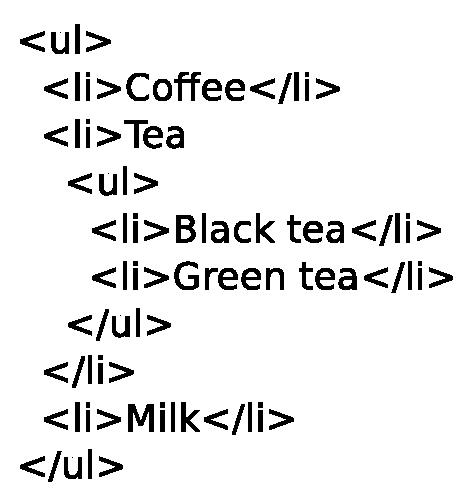
\epsfig{file=drawing/nestedHtmlList.eps,scale=0.65}
\caption{An example for nested HTML lists.}
\label{fig:nestedlist}
\end{figure}

\subsection{Candidate List Cleaning}
After extracting candidate lists from the top ranked search results, we further clean them as follows:
\begin{enumerate}[label={(\arabic*)}]
 \item First, all the list items are normalized by converting text to lowercase and removing non-alphanumeric characters.
 \item Then, we remove stopwords and duplicate items in each list.
 \item Finally, we discard all lists that contain only one item or more than 200 items. 
\end{enumerate}

After the cleaning process, we harvest a set of candidate lists, from which we want to build high-quality query facets. 

\section{Facet Refining}
\label{sec:facet-refine}
The candidate lists extracted are usually noisy~\cite{zhang2009employing},
and could be non-relevant to the issued query, therefore they cannot be used directly as query facets. For example, Table~\ref{tab:facet-candidates} shows four candidate lists extracted for the query \concept{baggage allowance}. $L_1$ contains terms that are relevant to \concept{baggage allowance}, but they are not coordinate terms -- \concept{delta}, \concept{france} and \concept{round-trip} are not members of the same class. 
$L_2$ is a valid query facet, but it is incomplete -- another airline \concept{aa} appears in $L_3$. $L_3$ is mixed with different facets, airlines and travel classes. $L_4$ is non-relevant to the query. 
\begin{table}[ht!]
\centering
\caption{Four candidate lists for the query \concept{baggage allowance}}
\label{tab:facet-candidates}
\begin{tabular}{|l|} \hline
 %Candidate facets \\ \hline
$L_1$: delta, france, round-trip\\
$L_2$: delta, jetblue, british airways\\ 
$L_3$: aa, first, business, economy\\
$L_4$: hard to remember, playing it by ear, ...\\
\hline
\end{tabular}
\end{table}

Since the candidate lists are frequently noisy, we need an effective way to refine extracted candidate lists into high-quality query facets. We call this problem \textbf{facet refining}, in which we take a set of candidate lists as input, and want to output high-quality query facets. This facet refining problem is the core issue in query facet extraction, and a main focus of this chapter. Existing query facet extraction models differ in how they refine candidate lists.

One related work about facet refining~\cite{dou2011finding} clusters similarity candidate lists together as query facets (called query dimensions in their original paper), and then ranks/selects clusters and cluster items based on heuristics scores. We find this method is difficult to incorporate features into. It also does not have the flexibility of breaking a candidate list into two query facets. We describe more about this method and other related method for facet refining in Section~\ref{sec:facet-other}. We also compare these methods with our models in Chapter~\ref{ch:intrinsiceval} and Chapter~\ref{ch:extrinsiceval}.

We instead treat the facet refining problem as a \textbf{selective clustering} problem. In the selective clustering problem, we do not cluster all given items, but only cluster a subset of the items. 
In the case of facet refining, we want to discard noisy terms, and cluster only facet terms in the candidate lists (\eg, \concept{aa}, \concept{delta}, \concept{jetblue}, \concept{british airways}, \concept{first}, \concept{business} and \concept{economy} in Table~\ref{tab:facet-candidates}) into query facets (\eg, \{\concept{aa}, \concept{delta}, \concept{jetblue}, \concept{british airways}\} and \{\concept{first}, \concept{business},\concept{economy}\}). We present this problem more formally in Section~\ref{sec:facet-formulation}.

To address this problem, we develop a supervised method based on a graphical model, presented in the next section.


\section{Query Faceting Models}
\label{sec:facet-gm}
In this section, we describe query faceting (QF) models, our supervised methods based on a directed graphical model for facet refining. A directed graphical model (or Bayesian network) is a graphical model that compactly represents a probability distribution over a set of variables ~\cite{pearl1988probabilistic}. It consists of two parts: 1) a directed acyclic graph in which each vertex represents a variable, and 2) a set of conditional probability distributions that describe the conditional probabilities of each vertex given its parents in the graph.

We treat facet refining as a selective clustering problem (as described in Section~\ref{sec:facet-refine}), and solve it as a labeling problem, in which we are trying to predict 1) whether a list item is a facet term, and 2) whether a pair of list items is in a same query facet. Then, we used a directed graphical model to exploit the dependences that exist between those labels. Similar to conditional random fields~\cite{lafferty2001conditional}, we directly model the conditional probability $P(y|x)$, where $y$ is the label we are trying to predict and $x$ is the observed data -- list items and item pairs. Thus, it avoids modeling the dependencies among the input variables $x$, and can handle a rich set of features. For our graph model, exact maximum a posteriori inference is intractable; therefore, we approximate the results using two algorithms.

In the rest of this section, we first describe the facet refining problem more formally in Section~\ref{sec:facet-formulation}, and then present our graphical model in Section~\ref{sec:facet-model}. We describe how to train and perform inference on the model in Section~\ref{sec:facet-train} and Section~\ref{sec:facet-infer} respectively.

\subsection{Problem Formulation}
\label{sec:facet-formulation}
Before diving into the QF method, we first define the facet refining problem more formally. We use $F=\{t_i\}$ to denote a query facet, consisting of a set of facet terms $t_i$. $\mathcal{F}=\{F_i\}$ denotes the set of query facets for the given query. $T_\mathcal{F}=\bigcup_i{F_i}$ denotes all the facet terms in $\mathcal{F}$. Candidate lists (or candidate facets) are just an imperfect version of query facets, and we substitute ``F'' with ``L'' to denote corresponding variables. $L=\{t_i\}$ denotes a candidate list. $\mathcal{L}=\{L_i\}$ denotes all the candidate lists extracted for the query. $T_\mathcal{L}=\bigcup_i{L_i}$ denotes all list items (or terms) in the candidate lists. Based on the formulation, the facet refining problem is simply to find $\mathcal{F}$ constrained with $T_\mathcal{F} \subseteq T_\mathcal{L}$, given $\mathcal{L}$ (and possibly other resources).

In our query faceting models, the facet refining problem was treated as a label prediction problem. It aims to learn and predict jointly 1) whether a list item is a facet term and 2) whether a pair of list items are in the same query facet. We denote the two types of labels as follows. The term/item labels are denoted by $Y=\{y_i\}$, where $y_i = 1\{t_i\!\in\! T_{\mathcal{F}}\}$ is a label indicating whether a list item $t_i$ is indeed a facet term. Here $1\{\cdot\}$ is the indicator function which takes on a value of 1 if its argument is true, and 0 otherwise. The pair labels are denoted by $Z=\{z_{i,j}\}$, where $z_{i,j} = 1\{\exists\, F\!\in\!\mathcal{F}, \, t_{i}\!\in\!F  \wedge  t_{j}\!\in\!F \}$ is a label indicates whether list item $t_i$ and $t_j$ are in the same query facet. Thus, the facet refining problem is now formulated as the problem of predicting labels $Y$ and $Z$.

\subsection{The Graphical Model}
\label{sec:facet-model}
Our supervised method is based on a directed graphical model, aiming to capture the dependencies between the term and pair labels. The graphical model is shown in Figure~\ref{fig:gm}. We further describe it as follows.

\begin{figure}[ht!]
\centering
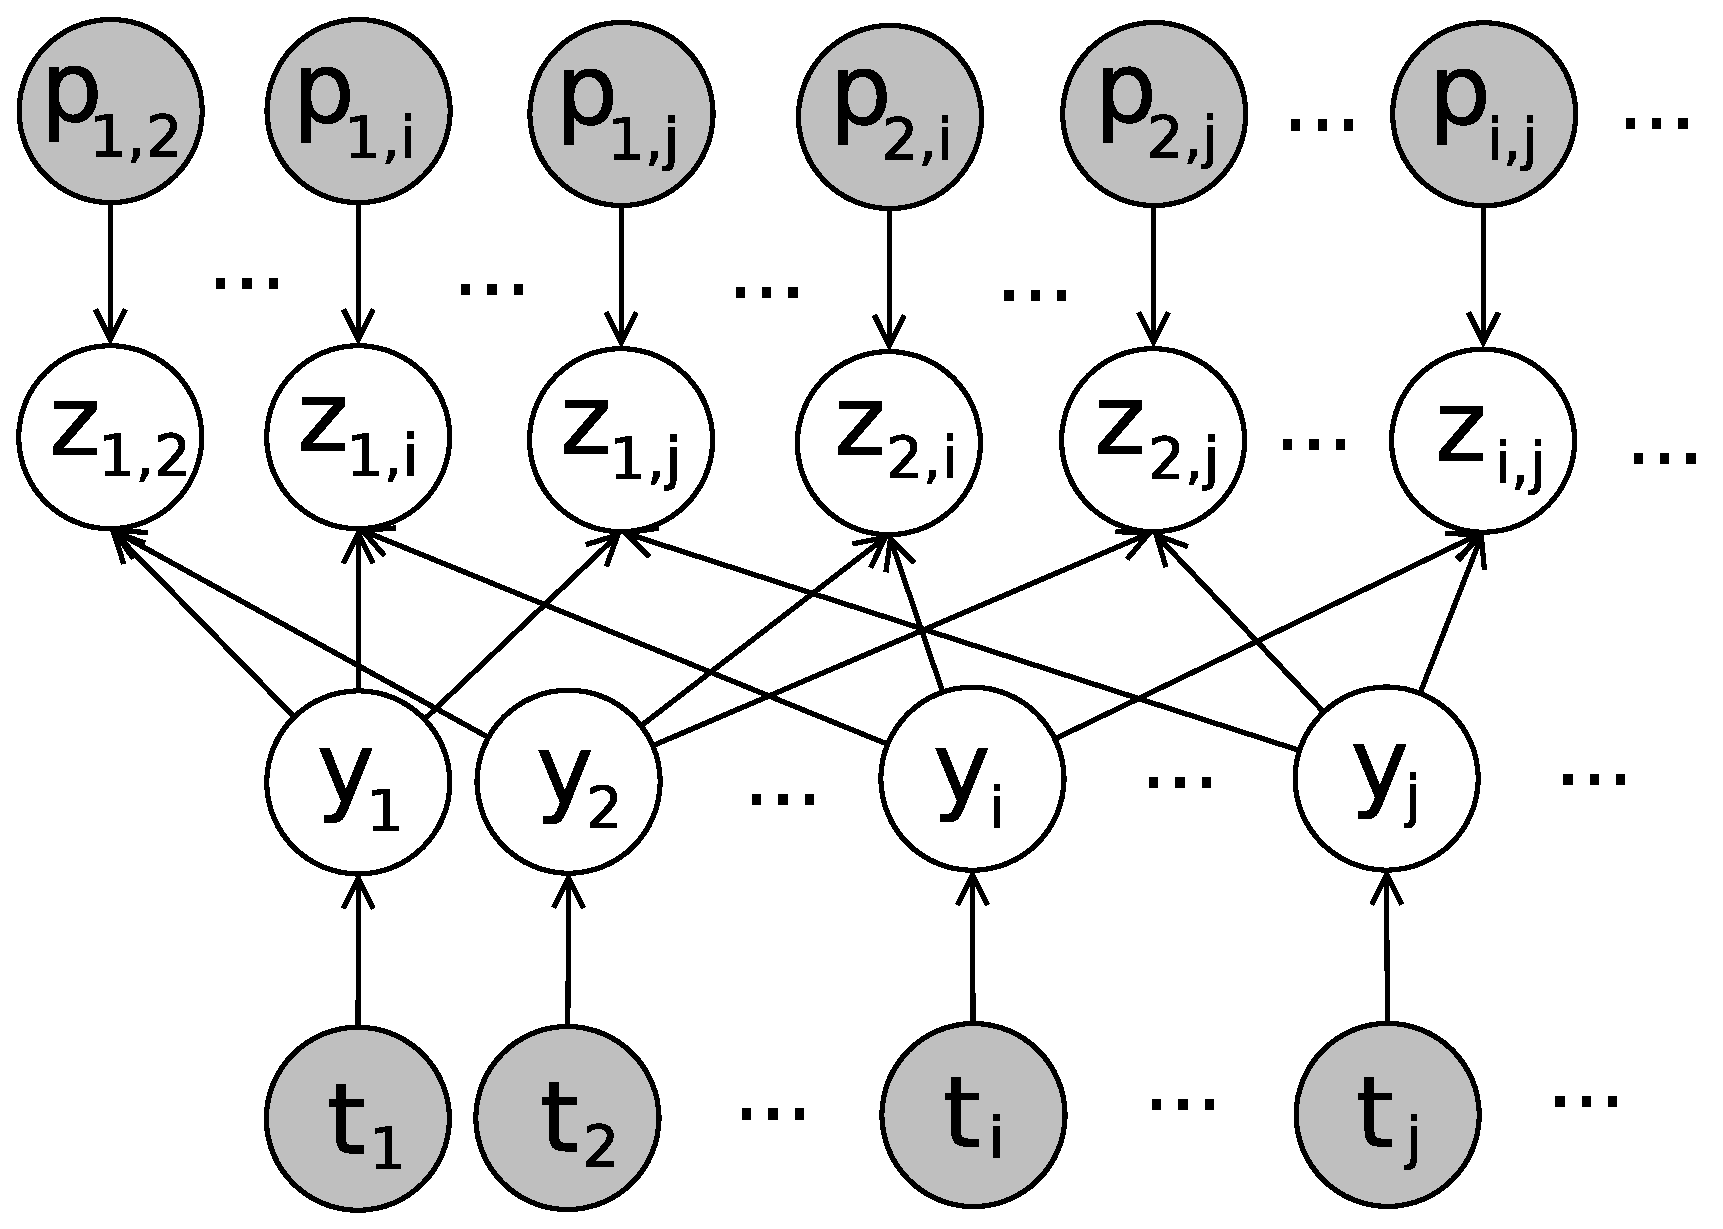
\epsfig{file=drawing/gm.eps,scale=0.25}
\caption{A graphical model for candidate list data}
\label{fig:gm}
\end{figure}

\subsubsection{The Graph}
First, we describes the four types of variables in the graphical model as follows. We use the formulation described in Section~\ref{sec:facet-formulation}.
\begin{itemize}
 \item list items: $t_i \in T_\mathcal{L}$, as defined before, are all the list items from the extracted candidate lists.
 \item item pairs: $p_{i,j}=(t_i,t_j)$ is simply a short name for term pair $t_i$ and $t_j$. $P_{\mathcal{L}}=\{p_{i,j}|\, t_i,t_j\!\in\!T_{\mathcal{L}}, \, t_i \!\neq\! t_j \}$ are all the item pairs in $T_\mathcal{L}$.
 \item item labels: $y_i \in Y$, as defined before, are all item labels.
  \item pair labels: $z_{i,j} \in Z$, as defined before, are pair labels.
\end{itemize}
List items $t_i$ and item pairs $p_{i,j}$ will be characterized by corresponding features (described in Section~\ref{sec:facet-features}). They are always observed. Item labels $y_i$ and pair labels $z_{i,j}$ are what we are trying to predict. In summary, the vertices in our graphical model are $V=T_{\mathcal{L}} \cup P_{\mathcal{L}} \cup Y \cup Z$.

Second, as shown in Figure~\ref{fig:gm}, there are three types of edges in the graph:
\begin{itemize}
 \item edges from each list item $t_i$ to its corresponding label $y_i$. 
 \item edges that point to each item pair label $z_{i,j}$ from the two corresponding list items $y_i$ and $y_j$.
 \item edges from each item pair $p_{i,j}$ to its corresponding label $z_{i,j}$.
\end{itemize}

\subsubsection{Conditional Probability Distributions}
We use logistic-based conditional probability distributions (CPDs) for variable $y_i$ and $z_{i,j}$, defined as in Equation~\ref{eq:y} and Equation~\ref{eq:z},
\begin{equation}
\label{eq:y}
P(y_i = 1|t_i)=\frac{1}{1+\exp\{-\sum_k{\lambda_k f_k(t_i)}\}},
\end{equation}
\begin{equation}
\label{eq:z}
P(z_{i,j} = 1|p_{i,j},y_i, y_j)=\frac{y_i y_j}{1+\exp\{-\sum_k{\mu_k g_k(p_{i,j})}\}},
\end{equation}
where $f_k$ and $g_k$ are features that characterize a list item and a item pair respectively. $\lambda$ and $\mu$ are the weights associated with $f_k$ and $g_k$ respectively. Compared to a conventional logistic function, Equation~\ref{eq:z} has an extra term, $y_iy_j$, in the numerator. When $y_i=0$ or $y_j=0$, we have $P(z_{i,j}=1|p_{i,j},y_i,y_j)=0$. This means when either of the two list items is not a facet term, the two items can never appear in a query facet together.
When both of the $t_i$ and $t_j$ are facet terms, $P(z_{i,j}=1|p_{i,j},y_i,y_j)$ becomes a conventional logistic function, which models the probability of $t_i$ and $t_j$ being grouped together in a query facet, given the condition that both $t_i$ and $t_j$ are facet term.

\subsubsection{Joint Conditional Probability}
Similar as in conditional random fields~\cite{lafferty2001conditional}, we directly model the joint conditional probability $P(Y,Z|T_{\mathcal{L}},P_{\mathcal{L}})$. Thus, it avoids modeling the dependencies among the input variables $T_{\mathcal{L}},P_{\mathcal{L}}$, and can handle a rich set of features. The joint conditional probability for the graphical model is calculated as
\begin{equation}
\label{eq:joint}
P(Y,Z|T_{\mathcal{L}},P_{\mathcal{L}}) = \prod_{i}{P(y_i|t_i)}\prod_{i,j}{P(z_{i,j}|p_{i,j},y_i, y_j)},
\end{equation}
where the $P(y_i|t_i)$ and $P(z_{i,j}|p_{i,j}, y_i, y_j)$ are defined in Equation~\ref{eq:y} and Equation~\ref{eq:z} respectively.

\subsubsection{Features}
\label{sec:facet-features}
There are two types of features used in our graphical model, term features and (term) pair features. 

\textbf{Item features}, $f_k(t)$ in the graphical model, characterize a single list item in terms of whether the item is a facet term. There are two factors we consider: (1) relevance to the query and (2) quality as a coordinate term. We design a rich set of features to capture the two factors from different perspectives. More specifically, the features we designed are based on different data sources, and based on different types of frequency counts as described in details below.

The different data sources we used include a large web corpus (ClueWeb09), the list item itself, and the top search result webpages. For the top search results, we consider extraction on the following fields/parts:
\begin{itemize}
 \item Content: the textual content of the search result webpages
 \item Title: the title of the search result webpages
 \item List: the candidate lists extracted from the search results. We also consider the candidate lists extracted by each extraction pattern (Section~\ref{sec:facet-candidate}) separately, as we find these patterns are of different extraction qualities (Section~\ref{sec:intrinsic-patterns}).
  \begin{itemize}
   \item Text: candidate lists extracted based on the lexical pattern
   \item Ol: candidate lists extracted based on the OL pattern
   \item Ul: candidate lists extracted based on the UL pattern
   \item Select: candidate lists extracted based on the SELECT pattern
   \item Tr: candidate lists extracted based on the TABLE pattern, and extracted by the rows.
   \item Td: candidate lists extracted based on the TABLE pattern, and extracted by the columns.
  \end{itemize}
\end{itemize}

We extract the following types of frequency counts (on the different fields) as features. Note that these frequency-based features are normalized using $log(frequency+1)$ \todo{explain why}.
\begin{itemize}
 \item Termfreq: item/term frequency, the frequency of the list item.
 \item PageFreq: page frequency, the number of search result webpages that contain the list item.
 \item WpageFreq: weighed PageFreq. Each search result webpage count is weighted by its rank, $1/\sqrt{rank}$. This assume that the webpages in the top ranks are more important.
 \item SiteFreq: site frequency, the number of unique websites of the search results that contain the list item. SiteFreq addresses the following problem of PageFreq. Some websites have a fixed template for all of its webpages.  Search results may contains multiple webpages from the same website. In that case, the candidate lists extracted from the template part may repeat multiple times, and be favored by PageFreq unreasonably.  
\end{itemize}

We list all item features in Table~\ref{tab:facet-tfeature}. To capture the relevance of list item (or term) to the query, we use some TF/IDF-based features extracted based on the search result content (Content), title (Title), a webpage corpus (Global corpus), and their combination (Combination). For example, \textit{ContentTermFreq} is the frequency count of the item in the text content of the top $k$ search results. \textit{TitleSiteFreq} is the number of webpages in the top $k$ search results that contain the item in their title. \textit{IDF} is the inverse document frequency of the list item based on a large web page corpus, ClueWeb09\footnote{http://lemurproject.org/clueweb09}. IDF is useful in down-weighting terms that occur frequently in generally, and thus likely to be less important. We calculate IDF as $IDF(t)=\log{\frac{N-N_{t}+0.5}{N_t+0.5}}$, where $N$ is the total number of documents in the collection, $N_t$ is the number of documents that contain $t$ (document frequency). We also combine 
different 
features together. For example, \textit{ContentTermFreq.IDF} multiples \textit{ContentTermFreq} with \textit{IDF} (like TF-IDF). \textit{ListTermFreq.ListIDF} multiples \textit{ListTermFreq} with \textit{ListIDF}, where \textit{ListTermFreq} is frequency count of the list item in the candidate lists extracted based on all the patterns. Besides relevance to the 
query and quality as coordinate terms, a facet term should also be succinct. Thus we also use feature \textit{Length}, which counts the number of words in the list item.


\begin{table}[h!]
\centering
\caption{Item features}
\label{tab:facet-tfeature}
\begin{tabular}{|c|c|l|l|}
\hline
\multicolumn{2}{|c|}{\textbf{Field/Source}}                &  \textbf{Feature} & \textbf{Description}\\ \hline
\multicolumn{2}{|c|}{\multirow{4}{*}{Content}}   & ContentTermFreq & TermFreq in Content\\ 
\multicolumn{2}{|l|}{}                    &  ContentPageFreq & PageFreq in Content \\  
\multicolumn{2}{|l|}{}                    &  ContentWpageFreq & WpageFreq in Content \\  
\multicolumn{2}{|l|}{}                    &  ContentSiteFreq & SiteFreq in Content \\ \hline  
\multicolumn{2}{|c|}{\multirow{3}{*}{Title}}   & TitleTermFreq & TermFreq in Title  \\ 
\multicolumn{2}{|l|}{}                    &  TitlePageFreq & PageFreq in Title \\  
\multicolumn{2}{|l|}{}                    &  TitleSiteFreq & SiteFreq in Title \\  \hline
		   \multirow{18}{*}{List} & \multirow{3}{*}{ListText} & ListTextTermFreq & TermFreq in ListText \\ 
						 &                   &  ListTextPageFreq & PageFreq in ListText \\ 
					         &                   &  ListTextSiteFreq & SiteFreq in ListText \\ \cline{2-4} 
                  & \multirow{3}{*}{ListOl} & ListOlTermFreq & TermFreq in ListOl \\ 
                  &                   &  ListOlPageFreq      & PageFreq in ListOl\\ 
                  &                   &  ListOLSiteFre       & SiteFreq in List\\ \cline{2-4} 
                  & \multirow{3}{*}{ListUl} & ListUlTermFreq  & TermFreq in ListUl \\ 
                  &                   &  ListUlPageFreq       & PageFreq in ListUl \\ 
                  &                   &  ListUlSiteFreq       & SiteFreq in ListUl \\ \cline{2-4} 
                  & \multirow{3}{*}{ListSelect} & ListSelectTermFreq  & TermFreq in ListSelect \\ 
                  &                   &  ListSelectPageFreq           & PageFreq in ListSelect \\ 
                  &                   &  ListSelectSiteFreq           & SiteFreq in ListSelect \\ \cline{2-4} 
                  & \multirow{3}{*}{ListTr} & ListTrTermFreq  & TermFreq in ListTr\\ 
                  &                   &  ListTrPageFreq       & PageFreq in ListTr \\ 
                  &                   &  ListTrSiteFreq       & SiteFreq in ListTr \\ \cline{2-4} 
                  & \multirow{3}{*}{ListTd} & ListTdTermFreq  & TermFreq in ListTd \\ 
                  &                   &  ListTdPageFreq       & PageFreq in ListTd \\ 
                  &                   &  ListTdSiteFreq       & SiteFreq in ListTd \\ \hline
\multicolumn{2}{|c|}{Term}                &  Length & number of words in the term \\ \hline
\multicolumn{2}{|c|}{\multirow{2}{*}{Global corpus}}   & IDF & inverse document frequency \\ 
\multicolumn{2}{|l|}{}                    &  ListIDF  & IDF in a candidate list collection \\  \hline
\multicolumn{2}{|c|}{\multirow{2}{*}{Combination}}   & ContentTermFreq.IDF &  ContentTermFreq $\times$ IDF \\ 
\multicolumn{2}{|l|}{}                    &  ListTermFreq.ListIDF & ListTermFreq $\times$ ListIDF \\  \hline
\end{tabular}
\end{table}


To capture how likely item $t$ is to be a coordinate term (or an instance of a semantic class), we use features extracted from candidate lists (List) based on different patterns (ListText, ListOl, ListUl, ListSelect, ListTr, ListTd). For example, \textit{listSelectTermFreq} is the frequency of the list item in the candidate lists extracted based on the SELECT pattern. \textit{listTextPageFreq} is the number of the search result webpages that contains the list item in candidate lists extracted based on the lexical pattern from the webpages. Some list items occur frequently in candidate lists across different queries, such as \textit{home}, \textit{contact us} and \textit{privacy policy}. They are treated as stopwords, and removed from the candidate lists. We also use \textit{listIDF} to cope with this problem, in a similar way as IDF.  \textit{listIDF} is the IDF of a list item in a collection of candidate lists we extracted (see Section~\ref{sec:ie-data}). It is calculated in the same form as \textit{IDF}, 
as $listIDF(t)=\log{\frac{NL-NL_{t}+0.5}{NL_t+0.5}}$, where $NL$ is the total number of candidate lists in the collection,  $NL_t$ is the number of lists contain the list item $t$.


\textbf{Item Pair Features}, $g(p_{i,j})$ in the graphical model, are used to capture how likely it is that a pair of list items should be grouped into a query facet, given that the two list item both are facet terms. We design item pair features based on different types of similarity between the two list items,  listed in Table~\ref{tab:facet-pfeature}. One straightforward feature is the frequency count of the two list items occurring in a same candidate list (\textit{ListCooccur}). Another one is the difference in the length of the list item (\textit{LengthDiff}), which assumes that similar list item should be of similar length. 

\begin{table}[h!]
\centering
\caption{Item pair features. $t_i$ and $t_j$ are an item pair.}
\label{tab:facet-pfeature}
\begin{tabular}{ |l|l| } \hline
  Feature  & Description \\ \hline
  LengthDiff  & Length difference in words, $|Length(t_i) - Length(t_j)|$ \\
  ListCooccur & Number of candidate lists in which $t_i$, $t_j$ co-occur\\
  TextContextSim & Similarity between text contexts\\
  ListContextSim & Similarity between list contexts\\
\hline
\end{tabular}
\end{table}


Besides these straightforward features, item similarity can also be measured by their context similarity. One common context for a term is the text content surrounding the term~\cite{shi2010corpus}. The feature based on text content similarity is called \textit{textContextSim} in Table~\ref{tab:facet-pfeature}. We build the text context using surrounding words (within 25 words) of the list item in the search result webpages, and represent the text context as a vector of term frequency weights, then we use cosine similarity to calculate \textit{TextContextSim}. Another context we propose in this work is based on the candidate lists extracted, which we call list context. We use list items that appears together with the given list item in the same candidate lists as the list context. An example is given in Table~\ref{tab:facet-listcontext}. In the example, the list context for \concept{Delta} include list item \concept{AA} (twice), \concept{JetBlue} (twice), \concept{Southwest}, and the list context for \
concept{
United} include list item \concept{AA}, \concept{JetBlue}, \concept{Southwest}. 
\begin{table}[ht!]
\centering
\caption{A list context example. $L1$, $L2$, $L3$ are three candidate lists. The list context for \concept{Delta} is marked by underline \underline{\textit{item}}, the list context for \concept{United} is marked by double-underline \uwave{item}.}
\label{tab:facet-listcontext}
\begin{tabular}{|l|} \hline
$L_1$: \underline{AA}, \textit{Delta}, \underline{JetBlue} \\
$L_2$: \underline{AA}, \textit{Delta}, \underline{JetBlue},  \underline{Southwest}\\
$L_3$: \uwave{AA}, \textit{United}, \uwave{JetBlue}, \uwave{Southwest}\\ 
\hline
\end{tabular}
\end{table}
Then we can calculate the similarity based on list context in the same way as \textit{TextContextSim} (\ie, using term frequency represent with cosine similar measure). This context similar feature is called \textit{ListContextSim}. \textit{ListContextSim} is to some extent similar to \textit{ListCooccur}, but one advantage of \textit{ListContextSim} is that even if two list items do not co-occur together in a candidate list, they may still have a high \textit{ListContextSim}. For the example in Table~\ref{tab:facet-listcontext}, \concept{Delta} and \concept{United} do not co-occur together in a candidate list, but their list contexts are very similar, and thus they obtain a high \textit{ListContextSim}.


\subsection{Maximum Likelihood Parameter Estimation}
\label{sec:facet-train}
We estimate the parameters $\lambda,\mu$ in the model by maximizing the conditional likelihood of a giving training set. (Later in Chapter~\ref{ch:precision}, we will present another method for parameter estimation by directly maximizing the performing measure.)
The training set for the graphical model can be denoted as
$\{T_{\mathcal{L}}^{(k)},P_{\mathcal{L}}^{(k)},Y^{*(k)},Z^{*(k)}\}$,
where $Y^{*(k)}$, $Z^{*(k)}$ are the ground truth labels for the list items $T_{\mathcal{L}}^{(k)}$ and item pairs $P_{\mathcal{L}}^{(k)}$. (We use superscript ``*'' to denote ground truth labels.)
The conditional probability of the training set can be calculated according to Equation~\ref{eq:train}.
\begin{equation}
\label{eq:train}
P(\lambda,\mu) = \prod_{k}{P(Y^{*(k)},Z^{*(k)}|T_{\mathcal{L}}^{(k)},P_{\mathcal{L}}^{(k)})},
\end{equation}
where $P(Y^{*(k)},Z^{*(k)}|T_{\mathcal{L}}^{(k)},P_{\mathcal{L}}^{(k)})$ is defined in Equation~\ref{eq:joint}. Based on the condition probability, the conditional log-likelihood $l(\lambda, \mu)$, can be calculated as follows,
\begin{equation}
\label{eq:ll}
l(\lambda,\mu) = l_t(\lambda) + l_p(\mu),
\end{equation}
\begin{equation}
\label{eq:lg1}
l_t(\lambda) = \sum_{k}{\sum_{i}{\log P(y_i^{*(k)}|t_i^{(k)})}} - \frac{\sum_{k}{\lambda_k^2}}{2 \sigma^2},
\end{equation}
\begin{equation}
\label{eq:lg2}
l_p(\mu) = \sum_{k}{\sum_{i,j}}{\log P(z_{i,j}^{*(k)}|p_{i,j}^{(k)},y_i^{*(k)},y_j^{*(k)})} -  \frac{\sum_{k}{\mu_k^2}}{2 \gamma^2},
\end{equation}
where the last terms in Equation~\ref{eq:lg1} and Equation~\ref{eq:lg2} are served as regularizers, which penalize large values of $\lambda$, $\mu$. $\sigma$ and $\gamma$ are regularization parameters that control the strength of penalty. 

Notice that, in the train set, for those item pairs $p_{i,j}$ with any of its list item not being a facet term, their labels $z_{i,j}^{*}=0$. According to Equation~\ref{eq:z}, for those item pairs, $\log P(z_{i,j}^{*}|p_{i,j},y_i^{*},y_j^{*})=0$, which makes no contribution to the conditional log-likelihood $l(\mu)$, and thus $l_p(\mu)$ can be simplified as
%\begin{equation}
%\label{eq:lg2x}
%l_p(\mu) = \sum_{T_{\mathcal{L}}}{\sum_{z_{i,j} \in Z'}{\log P(z_{i,j}|p_{i,j},y_i,y_j)}} -  \frac{\sum_{k}{\mu_k^2}}{2 \gamma^2}
%\end{equation}
\begin{equation}
\label{eq:lg2x}
l_p(\mu) = \sum_{k}{\sum_{i,j: y_i^{*(k)}=1, y_j^{*(k)}=1}}{\log P(z_{i,j}^{*(k)}|p_{i,j}^{(k)},y_i^{*(k)},y_j^{*(k)})} -  \frac{\sum_{k}{\mu_k^2}}{2 \gamma^2},
\end{equation}
where the $i,j$ now indexes only item pairs with both of its list items being facet terms (\ie,$y_i^{*(k)}=1, y_j^{*(k)}=1$).

We can see that Equations~\ref{eq:lg1} and \ref{eq:lg2x} are exactly the same as log-likelihoods for two separated logistic regressions. In fact, Equation~\ref{eq:lg1} learns a logistic regression model for whether a list item is a facet term, and Equation~\ref{eq:lg2x} learns a logistic regression model for whether two facet terms should be grouped together.
The parameter $\lambda$ and $\mu$ can be learned by maximizing the log-likelihood using gradient descent, exactly same as in logistic regression.
\todo{add gradient equations}
%Its partial derivatives can be calculated as follows,
%\begin{equation*}
%\label{eq:lg1p}
%\frac{\partial l(\lambda,\mu)}{\partial \lambda_k}  = \sum_{T_{\mathcal{L}}}{\sum_{y_i \in Y}{\left( y_i-P(y_i=1|t_i) \right) f_k(t_i)}} 
%- \frac{\lambda_k}{\sigma^2}
%\end{equation*}
%\begin{equation*}
%\label{eq:lg2p}
%\frac{\partial l(\lambda,\mu)}{\partial \mu_k}  = \sum_{T_{\mathcal{L}}}{\sum_{z_{i,j} \in Z'}{\left( z_{i,j}- %P(z_{i,j}=1|p_{i,j},y_i,y_j) \right) g_k(p_{i,j})}} 
%- \frac{\mu_k}{\gamma^2}
%\end{equation*}

\subsection{Inference}
\label{sec:facet-infer}
When given a new labeling task, we could perform maximum a posteriori inference -
compute the most likely labels $Y, Z$ by maximizing the joint conditional probability $P(Y,Z|T_{\mathcal{L}},P_{\mathcal{L}})$.
After that, the query facet set $\mathcal{F}$ can be easily induced from the labeling $Y, Z$.
(Collect list items with $y_i=1$ as facet terms, and group any two of them into a query facet if the corresponding $z_{i,j}=1$.)
Note that the graphical model we designed does not enforce the labeling to produce strict partitioning for facet terms.
For example, when $Z_{1,2}=1$, $Z_{2,3}=1$, we may have $Z_{1,3}=0$.
Therefore, the labeling results may induce an overlapping clustering.
Unfortunately, this optimization problem is NP-hard, which can be proved by a reduction from the Ising model~\cite{barahona1982computational}.

To facilitate developing solutions, we add the strict partitioning constraint that each facet term belongs to exactly one query facet. Also, to directly produce the query facets, instead of inducing them after predicting labels, we rephrase the optimization problem as follows. First, we use the following notations for log-likelihoods,\todo{clear up the equations}
\begin{eqnarray*}
 s_t(t_i) &=& \log P(y_i=1|t_i)      \nonumber \\
  \overline{s_t}(t_i)&=&\log \left( 1-P(y_i=1|t_i) \right) \nonumber \\
 s_p(t_i, t_j)&=&\log P(z_{i,j}=1|p_{i,j},y_i=1,y_j=1) \nonumber \\
  \overline{s_p}(t_i, t_j)&=&\log\left(1-P(p_{i,j}=1|p_{i,j},y_i=1,y_j=1)\right) \nonumber
\end{eqnarray*}
Using the notations above, the log-likelihood $l(\mathcal{F})$ for a particular query facet set $\mathcal{F}$ formed from $\mathcal{L}$ can be written as 
\begin{eqnarray}
\label{eq:target}
l(\mathcal{F}) &=&l_t(\mathcal{F}) + l_p(\mathcal{F}) \nonumber\\
l_t(\mathcal{F}) &=& \sum_{t\in T_\mathcal{F}}{s_t(t_i)}+\sum_{t\not\in T_\mathcal{F}}{\overline{s_t}(t_i)} \nonumber \\
l_p(\mathcal{F}) &=&\sum_{F \in \mathcal{F}}{\sum_{t_i,t_j \in F}{s_p(t_i,t_j)}} 
+ \sum_{\substack{F, F' \\ \in \mathcal{F}}}{\sum_{\substack{t_i \in F, \\ t_j \in F'}}{\overline{s_p}(t_i,t_j)}}
\label{eq:targetp}
\end{eqnarray}
In the right hand side of Equation~\ref{eq:targetp}, the first term  is the intra-facet score, which sums up $s_p(\cdot, \cdot)$ for all the item pairs in each query facet. The second term is the inter-facet score, which sums up the $\overline{s_p}(\cdot,\cdot)$ for each item pair that appears in different query facets. Then the optimization target becomes $\mathcal{F}=\arg\max_{\mathcal{F}\in\mathfrak{F}}{l(\mathcal{F})}$, where $\mathfrak{F}$ is the set of all possible query facet sets that can be generated from $\mathcal{L}$ with the strict partitioning constraint.

This optimization problem, however, is still NP-hard, which can be proved by a reduction from the Multiway Cut problem~\cite{bansal2002correlation}.
Therefore, we propose two algorithms, \textbf{QFI} and \textbf{QFJ}, to approximate the results.

\todo{add proof for NP-hardness}
\subsubsection{QFI}
QFI (Query Faceting Independent) approximates the results by predicting whether a list item is a facet term and whether two list items should be grouped in a query facet independently, which is accomplished in two phases.
In the first phase, QFI selects a set of list items as facet terms $T_\mathcal{F}$ according to $P(y_i|t_i)$.
In this way, the algorithm predicts whether a list item $t_i$ is a facet term independently, ignoring the dependences between $y_i$ and its connected variables in $Z$.
In our implementation, we simply select list items $t_i$ with  $P(t_i)> w_{min}$ as facet terms. (For convenience, we use $P(t_i)$ to denote $P(y_i=1|t_i)$.)
In the second phase, the algorithm clusters the facet terms $T_\mathcal{F}$ selected in the first phase into query facets, according to $P(t_i,t_j)$, where $P(t_i, t_j)$ is used to denote $P(z_{i,j}=1|p_{i,j},y_i=1,y_j=1)$. Using $P(t_i,t_j)$ as the distance measure, many clustering algorithm can be applied here.
For our implementation, we use a cluster algorithm based on WQT (Quality Threshold with Weighted items)~\cite{dou2011finding}, because it considers the importance of terms while clustering.
We use $P(t_i)$ as the measure for facet term importance, and $dist_t(t_i,t_j)=1-P(t_i, t_j)$ as the distance measure for facet terms. The distance between a cluster and a facet term is computed using complete linkage distance, $dist_f(F,t)=max_{t' \in F}{d_t(t, t')}$, and the diameter of a cluster can be calculated as $dia(F)=\max_{t_i,t_j\in F}{dist_t(t_i,t_j)}$. 

Algorithm QFI is shown in Algorithm~\ref{alg:qfi}. It takes the thresholds for term probability $w_{min}$ and cluster diameter $dia_{max}$ as inputs, as well as measure functions for term importance $P(t)$, distance $dist_f(F,t)$ and cluster diameter $dia(F)$. First, it selects facet terms by thresholding $P(t)$ (Line~\ref{alg:qfi-term}). Then it initializes the facet term pool to be clustered (Line~\ref{alg:qfi-pool}), and sets the return result as an empty set (Line~\ref{alg:qfi-fempty}). After that, it processes the facet terms in decreasing order of $P(t)$, and builds a cluster for each of them (Line~\ref{alg:qfi-while1} to \ref{alg:qfi-while1-e}). For each facet term, it builds a cluster by iteratively adding the facet term that is closest to the cluster (Line~\ref{alg:qfi-closest}), until the diameter of the cluster surpasses the threshold $dia_{max}$ (Line~\ref{alg:qfi-dia}). Last, clusters are collected (Line~\ref{alg:qfi-collect}) and returned (Line~\ref{alg:qfi-return}).

\begin{algorithm}[ht!]
 \caption{QFI}
\label{alg:qfi}
\begin{algorithmic}[1]
  \Require $w_{min}, dia_{max}, P(t), dist_f(F,t), dia(F)$
  \Ensure $\mathcal{F}$
  \State $T_\mathcal{F} \leftarrow \{t\;|\;P(t)\!>\!w_{min}\}$ \label{alg:qfi-term}
  \State $T_{pool} \leftarrow T_\mathcal{F}$ \label{alg:qfi-pool}
  \State $\mathcal{F} \leftarrow \emptyset$ \label{alg:qfi-fempty}
  \While{$T_{pool} \neq \emptyset$} \label{alg:qfi-while1}
    \State $t \leftarrow \arg\!\max_{t\in T_{pool}}{P(t)}$ 
    \State $F \leftarrow \{t\}$
    \State $T_{pool}\leftarrow {T_{pool}}\!-\!\{t\}$
    \While{$T_{pool} \neq \emptyset$}
      \State $t' \leftarrow \arg\!\min_{t'\in T_{pool}}{dist_f(F,t')}$ \label{alg:qfi-closest}
      \If{$dia(F \cup \{t'\}) > dia_{max}$} \label{alg:qfi-dia}
	\State \textbf{break}
      \EndIf
      \State $F \leftarrow F \cup \{t'\}$
      \State $T_{pool}\leftarrow {T_{pool}}\!-\!\{t'\}$
    \EndWhile
    \State $\mathcal{F} \leftarrow \mathcal{F} \cup \{F\}$ \label{alg:qfi-collect}
  \EndWhile \label{alg:qfi-while1-e}
  \State \Return $\mathcal{F}$ \label{alg:qfi-return}
\end{algorithmic}
\end{algorithm}

QFI contains two parameters $w_{min}$, $dia_{max}$. They can be tuned for optimizing a given performance measure. QFI is also efficient. The dominant procedure for time complexity is the clustering part (Line~\ref{alg:qfi-while1} to ~\ref{alg:qfi-while1-e}). In clustering, each facet term is considered only once for forming a cluster or being added to a cluster. When considering adding a facet term to a cluster, it takes $O(m)$ time to calculate the distance $dist_f(F,t)$, where $m$ is the number of facet terms in the $F$. $m$ is bounded by the total number of facet terms selected, $n$. Therefore, overall QFI takes $O(n^2)$ time.

\subsubsection{QFJ}
QFI finds query facets based on the graphical model by performing inference of $y_i$ and $z_{i,j}$ independently.
The second algorithm, QFJ (Query Faceting Joint), instead tries to perform joint inference by approximately maximizing our target $l(\mathcal{F})$ with respect to  $y_i$ and $z_{i,j}$ iteratively.
The algorithm first guesses a set of list items as facet terms.
Then it clusters those facet terms by approximately maximizing $l_p(\mathcal{F})$, using a greedy approach. 
After clustering, the algorithm checks whether each facet term ``fits'' in its cluster, and removes those that do not fit.
Using the remaining facet terms, the algorithm repeats the process (clustering and removing outliers) until convergence.

QFJ is outlined in Algorithm~\ref{alg:qfj}. The inputs to the algorithm include the candidate list item set $T_{\mathcal{L}}$, term probability $P(t)$, the log-likelihoods $l(\mathcal{F})$, $l_p(\mathcal{F})$.
First, we select top $n$ list items according to $P(t)$ as the initial facet terms (Line~\ref{alg:qfj-term}), because it is less sensitive to the absolute value of the probabilities.
In our experiment, $n$ is set to 1000 to make sure most of the correct facet terms are included.
Then, the algorithm optimizes $l(\mathcal{F})$ by iteratively performing functions \textproc{Cluster} and \textproc{RemoveOutliers}.

\begin{algorithm}[h!]
 \caption{QFJ}
\label{alg:qfj}
\begin{algorithmic}[1]
  \Require $T_{\mathcal{L}}, P(t), l(\mathcal{F}), l_p(\mathcal{F}), n$
  \Ensure $\mathcal{F}=\{F\}$
  \State $T_\mathcal{F} \leftarrow$ top $n$ list items from $T_{\mathcal{L}}$ according to $P(t)$ \label{alg:qfj-term}
  \Repeat
  \State $\mathcal{F}\leftarrow$ \Call{Cluster}{$T_{\mathcal{F}},l_p$}
  \State $T_\mathcal{F}\leftarrow$ \Call{RemoveOutliers}{$\mathcal{F},l$}
  \Until converge
  \State \Return $\mathcal{F}$
  \State
  \Function{cluster}{$T_\mathcal{F}, l_p$}
    \State $\mathcal{F} \leftarrow \emptyset$ 
    \For {each $t \in T_\mathcal{F}$ in decreasing order of $P(t)$} \label{alg:cluster-b}
      \State choose to put $t$ into the best facet in $\mathcal{F}$ 
      \State or add $t$ as a singleton into $\mathcal{F}$, 
      \State whichever has the highest resulting $l_p(\mathcal{F})$.
      %\For {each $F \in \mathcal{F}$}
	%\State $\Delta_{1}(F)\leftarrow \sum_{t' \in F}{\left(s_p(t,t')-\overline{s_p}(t,t')\right)}$ 
      %\EndFor
      %\If{$\max_{F}{\Delta_{1}(F)} < 0$}
	%\State $F' \leftarrow \{t\}, \mathcal{F}\leftarrow \mathcal{F} \cup \{F'\}$
      %\Else
      %\State find the best facet, $F_{best} \leftarrow \arg\max_F{\Delta_{1}(F,t)}$
      %\State add $t$ to the facet in $\mathcal{F}$, $F_{best} \leftarrow F_{best} \cup \{t\}$
      %\EndIf
    \EndFor \label{alg:cluster-e}
  \State \Return $\mathcal{F}$
  \EndFunction 
  \State
\Function{RemoveOutliers}{$\mathcal{F},l$}
  \State $T_\mathcal{F}\leftarrow$ all facet terms in $\mathcal{F}$
  \For {each $F \in \mathcal{F}$}
    \State $F'=\emptyset$
    \For {each $t \in F$ in decreasing order of $P(t)$} \label{alg:qfj-check}
      \State choose to add $t$ into $F'$ or not,
      \State whichever has the highest resulting $l(\{F'\})$
      \State if not, $T_\mathcal{F}\leftarrow T_\mathcal{F} - \{t\}$ \label{alg:qfj-remove}
      %\State $\Delta_{2} = \overline{s_t}(t) - s_t(t) - \sum_{t'\in F'}{s_p(t,t')} $
      %\If {$\Delta_{2} > 0$}
	%  \State remove $t$ from the facet in  $\mathcal{F}$, $F \leftarrow F - \{t\}$
      %\Else
	%  \State $F' \leftarrow F' \cup \{t\}$
      %\EndIf
    \EndFor
  \EndFor
  \State \Return  $T_\mathcal{F}$ \label{alg:qfj-return}
\EndFunction 
\end{algorithmic}
\end{algorithm}

\textproc{Cluster} performs clustering over a given set of facet terms.
In Line~\ref{alg:cluster-b} to \ref{alg:cluster-e}, it puts each facet terms into a query facet by greedily choosing the best facet, or creates a singleton for the list item, according to the resulting log-likelihood, $l_p(\mathcal{F})$.
%In step 5, $\Delta_{1}(F)$ is the difference between $l(\mathcal{F})$'s changes of adding the list item $t$ to $F$ and creating a singleton for $t$.
We choose to process these list items in decreasing order of $P(t)$, because it is more likely to form a good query facet in the beginning by doing so.

\textproc{RemoveOutliers} removes outlier facet terms in the clusters according to the joint log-likelihood $l(\mathcal{F})$. Initially, $T_\mathcal{F}$ contains all facet terms in $\mathcal{F}$ (Line~\ref{alg:qfj-term}). Then, for each cluster in $\mathcal{F}$, the function checks each facet term inside it (Line~\ref{alg:qfj-check}) to see if the facet term fits in the cluster according to the likelihood $l(\{F'\})$. If the facet term does not fit in the cluster (\ie, the facet term is an outlier), the function removes it from $T_\mathcal{F}$ (Line~\ref{alg:qfj-remove}). Last, the function returns the remaining facet terms in $T_\mathcal{F}$ (Line~\ref{alg:qfj-return}), which will be re-clustered in \textproc{Cluster}.
%$F'$ is the set of facet terms the algorithm selected when processing each facet $F$.
%In step 7 to 12, the algorithm chooses the best option for $t$ to maximize the log-likelihood $l(\mathcal{F})$. The list items we select from step 2 may contain ``bad'' facet terms. In step 14 to 24, the algorithm tries to delete those mistakes by locally optimize $l(\{F\})$ for each query facet $F$ formed. For each facet $F$, it consider whether each list item in the list should be delete or not. In step 15, $F'$ is the set of list items that we think should be kept after processing. $\Delta_2$ is the difference between $l(\{F'\})$'s changes of not including $t$ in $F'$ and including $F'$.

The parameter $n$ is set to a large number (1000 in our experiments) to ensure not missing facet terms initially, and thus it is not used as a tuning parameter. Therefore, different from QFI, QFJ does not have tuning parameters for optimizing a given performance measure. Instead, QFJ is purely guided by the log-likelihood object in the inferencing procedure. In terms of time complexity QFJ is close to QFI. \textproc{Cluster} processes each of the $n$ facet terms. For each facet term, it considers $k$ potential query facets to add the facet term. For each query facet option, the computation for the resulting $l_p(\mathcal{F})$ takes $O(n)$ time. Thus, overall \textproc{Cluster} takes $O(kn^2)$ time. \textproc{RemoveOutliers} considers to remove each of the $n$ facet term as an outlier only once. In considering removing a facet term, computing $l\{F'\}$ takes $O(n)$ time. Thus, the overall time complexity for \textproc{RemoveOutliers} is $O(n^2)$. QFJ repeats \textproc{Cluster} and \textproc{RemoveOutliers} until convergence, thus QFJ takes $O(r \cdot k n^2)$ time, where $r$ is the number of iterations. In practice, we find $r$ and $k$ are small. Thus, the time complexity for QFJ is similar to QFI.


\subsection{Ranking Query Facets}
The output of QFI and QFJ is a set of query facets $\mathcal{F}$. To produce ranking results, we defined a score for a query facet as $score_F(F)=\sum_{t \in F}{P(t)}$, and rank the query facets according to this scoring, in order to present more facet terms in the top. Facet terms within a query facet are ranked according to $score_t(t)=P(t)$. We leave the investigation for more sophisticated ranking models as future work.

\section{Other Approaches}
\label{sec:facet-other}
In this section, we describe two alternative method for facet refining. They are used as baselines in our experiments. 

\subsection{QDMiner}
\citet{dou2011finding} developed QDMiner/QDM for query facet extraction, which appears to be the first work that addressed the problem of query facet extraction.
To solve the problem of finding query facets from the noisy candidate lists extracted, they used an unsupervised clustering approach.
It first scores each candidate list by combining some TF/IDF-based scores.
The candidate lists are then clustered with bias toward important candidate lists, 
using a variation of the Quality Threshold clustering algorithm~\cite{heyer1999exploring}.
After clustering, clusters are ranked and list items in each clusters are ranked/selected based on some heuristics.
Finally, the top $k$ clusters are returned as results.
%They applied clustering on the candidates lists, and ranked/selected clusters and list items in those clusters based on some heuristics.
This unsupervised approach does not gain by having human labels available.
Also, by clustering lists, they lose the flexibility of breaking a candidate list into different query facets.

\subsection{Topic modeling}
In semantic class extraction, \citet{zhang2009employing} proposed to use topic models 
to find high-quality semantic classes from a large collection of extracted candidate lists.
Their assumption is, like documents in the conventional setting, candidate lists are generated by a mixture of hidden topics, which are the query facets in our case. pLSA and LDA are used in their experiments.
We find this approach can be directly used for finding query facets from candidate lists.
The major change we need to make is that: in semantic class extraction, topic modeling is applied globally on the candidate lists (or a sample of them) from the entire corpus; in query facet extraction, we apply topic modeling only on the top $k$ search results $\mathcal{D}$, assuming the coordinate terms in $\mathcal{D}$ are relevant to the query.
Then, the topics are returned as query facets, by using the top $n$ list items in each topic (according to the list item's probability in the topic).
Though this topic modeling approach is more theoretically motivated, it does not have the flexibility of adding different features to capture different aspects such as query relevance.

\section{Summary}
In this chapter, we developed query facet extraction, which extracts facets for a given query from its search results. We developed a supervised approach based on a graphical model to recognize facets from the noisy candidates found. The graphical model learns how likely a candidate term is to be a facet term as well as how likely two terms are to be grouped together in a query facet, and captures the dependencies between the two factors. We proposed two algorithms (\QFI and \QFJ) for approximate inference on the graphical model since exact inference is intractable. Compared with other existing methods, our models can easily incorporate a rich set of features, and learn from available labeled data.

To evaluate our models, in the next chapter, we develop an intrinsic evaluation method that compares extracted facets with human created ones.
